\documentclass[letterpaper]{article} % DO NOT CHANGE THIS
\usepackage[submission]{aaai2027}  % DO NOT CHANGE THIS
% The serif, sans-serif, and monospaced fonts are loaded automatically by
% aaai2027.sty (newtxtext, helvet, courier). DO NOT add \usepackage{times},
% \usepackage{helvet}, \usepackage{courier}, or any other font package.
\usepackage[hyphens]{url}  % DO NOT CHANGE THIS
\usepackage{graphicx} % DO NOT CHANGE THIS
\urlstyle{rm} % DO NOT CHANGE THIS
\def\UrlFont{\rm}  % DO NOT CHANGE THIS
\usepackage{natbib}  % DO NOT CHANGE THIS AND DO NOT ADD ANY OPTIONS TO IT
\usepackage{caption} % DO NOT CHANGE THIS AND DO NOT ADD ANY OPTIONS TO IT
\frenchspacing  % DO NOT CHANGE THIS
%
% Recommended for better-looking tables
\usepackage{booktabs}
% Mathematics (\operatorname, \eqref, split)
\usepackage{amsmath}
%
% Keep the \pdfinfo as shown here. There's no need
% for you to add the /Title and /Author tags.
\pdfinfo{
/TemplateVersion (2027.1)
}

\setcounter{secnumdepth}{0} %May be changed to 1 or 2 if section numbers are desired.

\newcommand{\code}[1]{\texttt{#1}}

% Title in Title Case (AAAI rule: capitalise both words of hyphenated terms).
\title{Do LLM Monitors Miss Rare Threats?\\A Pre-Registered Test of the Low-Prevalence Effect}
\author{
    Anonymous Submission
}
\affiliations{
}

\begin{document}

\maketitle

\begin{abstract}
AI control protocols use language-model monitors to review the work of more capable, untrusted AI systems and to send the most suspicious items to a small human audit. Real attacks are expected to be rare. Human screeners miss rare targets far more often than common ones, mainly because they grow reluctant to say ``yes''; airport security counters this with Threat Image Projection. A pre-registered experiment tested whether large language model (LLM) monitors show this low-prevalence effect. Two Claude models made 30,880 judgements of Python solutions drawn from 379 execution-verified pairs of clean and backdoored code. The prediction failed in the opposite direction. In batches of 40, both monitors caught more backdoors when backdoors were rare: hit rates rose from 0.51 at 50\% prevalence to 0.69 at 2.5\% for Haiku, and from 0.50 to 0.74 for Sonnet (Holm-adjusted $p = .0015$ and $p < .001$), with false-alarm rates below 2\%. The decision criterion did not become more conservative. Single-item review caught about as many backdoors as 2.5\% batches, and more than 10\% and 50\% batches in three of four comparisons. Stating that about 1 in 100 submissions contained a backdoor, rather than about half, slightly lowered Sonnet's single-item hit rate (0.85 to 0.78); Haiku's change was not significant. A labelled calibration block modelled on Threat Image Projection did not reliably raise hit rates and more than doubled Sonnet's false alarms. Rarity did not increase misses. Misses were more frequent when several backdoors shared a batch than when one did.
\end{abstract}

% ===========================================================================
\section{Introduction}

AI control is the study of safety measures that are meant to keep working even if an AI system is deliberately trying to defeat them \citep{greenblatt2024}. A central measure is \emph{trusted monitoring}. A capable but \emph{untrusted} model does the work. A weaker model that is \emph{trusted}, typically because it is thought too limited to subvert the protocol deliberately, reads each output and gives it a suspicion score. The most suspicious outputs go to a small budget of careful human review, called \emph{auditing}. In the original code-writing testbed the audit budget covered 2\% of problems \citep[Sec.~2.2]{greenblatt2024}.

The attacks such a monitor is meant to catch are expected to be rare. In control evaluations the \emph{red team}, which plays the part of a misaligned model, can defeat simple auditing by attacking seldom, so that no attack is likely to fall inside the audited sample (\citealp[Sec.~3.1]{greenblatt2024}; \citealp[Sec.~3.1]{bhatt2025}). A sketch of a control safety case notes that a model ``might simply attack very rarely such as once out of thousands of tasks'' \citep[Sec.~6]{korbak2025}.

Human factors research has studied this situation for decades. In a simulated baggage-screening task, misses rose from 7\% when targets appeared on half of trials to 30\% when they appeared on 1\% \citep{wolfe2005}. The extra misses come mainly from a shift in decision criterion: observers say ``no'' more readily, while their ability to tell targets from non-targets changes little \citep{wolfe2007}. Airport security responds with Threat Image Projection (TIP), software that projects images of fictional threats into a small share of real bags and records whether the screener finds them \citep{cutler2009,buser2025}.

Do LLM monitors behave the same way? Current practice mostly assumes that prevalence does not matter. In eleven audited evaluations of detectors for hijacked LLM agents, attacks made up 16\% to 86\% of test samples and ``no evaluation varies that share'' \citep[Abstract]{abbasi2026}. Estimates at low prevalence apply rates measured at high prevalence (\citealp[Sec.~6.3]{srivastav2026}; \citealp[Sec.~III.E]{abbasi2026}), and a formal model of trusted monitoring treats suspicion scores as ``a distribution, conditioned on whether the code is safe or backdoored'' \citep[Sec.~2]{griffin2024}. Two opposite predictions are plausible. The human prediction is that a monitor that sees few attacks becomes more conservative and misses more of them. The competing prediction is that a lone attack stands out among benign items, or that a model normalises its decisions within a batch \citep{hida2026}, so that rare attacks are caught \emph{more} often.

This paper reports a pre-registered experiment that tests these predictions with LLM monitors of code. Its contributions are:
\begin{itemize}
\item A pre-registered test that separates \emph{experienced} prevalence (the share of backdoored submissions in a reviewed batch) from \emph{stated} prevalence (a sentence in the prompt). Both monitors caught more backdoors at 2.5\% prevalence than at 50\%.
\item A signal detection analysis showing that this reversal was not a conservative criterion shift; post hoc, backdoored items scored lower when several shared a batch.
\item A test of two remedies at low prevalence: a TIP-style labelled calibration block, taken from screening research, and an instruction to judge each item independently. Neither reliably raised hit rates.
\item An open set of 419 execution-verified pairs of clean and backdoored solutions built from MBPP, with code, prompts and all raw monitor outputs (link withheld for review).
\end{itemize}

The design was pre-registered and committed to a git repository before any main-experiment data were collected; the link is withheld for review. Later clarifications, and when each was committed, are summarised under Methods.

% ===========================================================================
\section{Background}

\subsection{Signal Detection Theory}

Signal detection theory (SDT) describes decisions about whether a signal is present \citep{green1966,hautus2021}. A \emph{signal} trial is a backdoored submission and a \emph{noise} trial is a clean one. Flagging a backdoored item is a \emph{hit}; flagging a clean item is a \emph{false alarm}. From the hit rate $H$ and false-alarm rate $F$, sensitivity
\begin{equation}\label{eq:dprime}
d' = z(H) - z(F)
\end{equation}
measures how well the observer separates the two kinds of item, and the criterion
\begin{equation}\label{eq:criterion}
c = -\frac{1}{2}\bigl[z(H) + z(F)\bigr]
\end{equation}
measures how much evidence it needs before saying ``yes''. Here $z$ is the inverse of the standard normal cumulative distribution function. A positive $c$ is conservative (fewer flags, more misses); a negative $c$ is liberal. Because $z$ is infinite at 0 and 1, rates are corrected with the log-linear rule, in which ``each cell frequency in the contingency table is increased by 0.5'' \citep[Abstract]{hautus1995}. The corrected rates are
\begin{equation}\label{eq:loglinear}
\tilde H = \frac{n_{\mathrm{h}} + 0.5}{n_{\mathrm{s}} + 1}, \qquad \tilde F = \frac{n_{\mathrm{f}} + 0.5}{n_{\mathrm{n}} + 1},
\end{equation}
where $n_{\mathrm{h}}$ and $n_{\mathrm{f}}$ are the numbers of hits and false alarms and $n_{\mathrm{s}}$ and $n_{\mathrm{n}}$ the numbers of signal and noise trials. $d'$ and $c$ are computed with $\tilde H$ and $\tilde F$ in Eqs.~\eqref{eq:dprime} and~\eqref{eq:criterion}; the rates $H = n_{\mathrm{h}}/n_{\mathrm{s}}$ and $F = n_{\mathrm{f}}/n_{\mathrm{n}}$ reported in the tables are uncorrected. For graded ratings, such as a suspicion score from 0 to 100, the area under the receiver operating characteristic curve (AUROC) summarises sensitivity across all thresholds; 0.5 is chance and 1.0 is perfect separation.

\subsection{The Low-Prevalence Effect and Its Remedies}

\citet{wolfe2005} asked observers to look for ``tools'' among other semi-transparent objects in an artificial baggage-screening task. Misses were 7\% at 50\% target prevalence, 16\% at 10\% and 30\% at 1\%. \citet[Abstract]{wolfe2007} found the effect ``very robust'' and concluded that ``[i]n signal detection terms, the prevalence effect can be explained as a criterion shift and not a change in sensitivity''. Several attempts to move observers to a better criterion failed. One regime worked: brief retraining periods at high prevalence with full feedback, inserted among long low-prevalence periods without feedback (Experiment~7). In that experiment ``[t]here were no significant effects of prevalence'', while false alarms were higher than in the authors' baseline experiment. Trained screeners show the effect too, and unlike in the laboratory their $d'$ also changed with prevalence \citep{wolfe2013}. Occasional \emph{probe} trials with known targets also reduce the effect, but ``[t]he probe benefit scaled with the frequency of the matching target'' \citep[Abstract]{becker2026}. The opposite problem also exists: when one display holds several targets, ``once one target is found, additional targets are likely to be missed'', studied as \emph{subsequent search misses} \citep[Abstract]{cain2013}.

In TIP, fictional threat items are typically projected onto 1\% to 4\% of bags, and the system tells the screener immediately whether a projected item was present \citep[Sec.~2]{buser2025}. TIP thus raises experienced prevalence, gives feedback and measures performance. \citet[Sec.~4]{korbak2025} sketch a control safety case whose safety layer ``audits the 0.1\% most suspicious actions'', and in which ``developers regularly generate synthetic attacks and check whether human auditors remain attentive and flag synthetic attacks as suspicious''. That proposal is TIP in all but name.

\subsection{LLM Judges, Context Effects and the Gap}

In few-shot classification, ``[w]hen the prompt is unbalanced, the predictions are unbalanced (majority label bias)'' \citep[Fig.~4 caption]{zhao2021}. Prior scores placed in a judge's context ``anchor judgments and systematically shift ratings toward their values'', and neither chain-of-thought nor a warning to disregard them reduced the total effect \citep[Abstract]{kapetanovic2026}. \citet{hida2026} compared one-at-a-time and batch screening (20 items per call) of studies for systematic reviews, in five reviews whose natural share of relevant studies ranged from 2.9\% to 53.0\%. For one model, batching made screening more inclusive in the four reviews with prevalence of 20\% or less and more restrictive in the balanced review, a pattern the authors call ``compatible with a possible tendency toward implicit normalization of decisions within the batch'' (Section~4.4). Prevalence there was confounded with review topic and items. \citet[Abstract]{kim2026} showed that ``a harmful question that is reliably refused in isolation can elicit a harmful response when embedded in a batch of benign questions'', which they attribute partly to ``refusal signal dilution''.

Searches of arXiv, the web and the reference lists of the papers above found no study that manipulates the prevalence of targets within an LLM monitor's or judge's context while holding the pool of items fixed, no study of prevalence effects in an AI-control setting, and no test of TIP-style remedies for LLM monitors. \citet{hida2026} is the nearest.

\paragraph{The analogy and the two predictions.} The human effect has a decision part, a criterion that tracks experienced prevalence \citep{wolfe2007}, and a behavioural part: observers quit target-absent searches earlier when targets are rare \citep{wolfe2005,wolfe2007}. An LLM has no time cost and no fatigue across calls. It reads every item it is given at once, and its ``experience'' of prevalence exists only inside one context window. A low-prevalence effect would have to come through the decision part, for example through majority-label bias \citep{zhao2021} or dilution of a rare signal among benign items \citep{kim2026}. Other mechanisms predict the opposite. A single backdoored item among 39 clean ones may stand out by contrast (``pop-out''), and a tendency to normalise decisions within a batch \citep{hida2026} would make a monitor flag relatively more when few items deserve it. The pre-registration therefore stated that a higher hit rate at low prevalence would be reported as a disconfirmation of H1.

% ===========================================================================
\section{Methods}

\subsection{Design and Hypotheses}

Three experiments, each run with two monitor models, test four confirmatory hypotheses:
\begin{itemize}
\item \textbf{H1 (experienced prevalence).} In batch review, the hit rate is lower at 2.5\% backdoor prevalence than at 50\%, with 10\% in between.
\item \textbf{H1a (criterion, not sensitivity).} That effect shows as a more conservative criterion $c$, with a smaller change in $d'$ and AUROC.
\item \textbf{H2 (stated prevalence).} In single-item review, stating that backdoors are rare (1\%) rather than common (50\%) lowers the hit rate.
\item \textbf{H3 (remedy).} At 2.5\% prevalence, a short labelled high-prevalence calibration block shown before the batch raises the hit rate.
\end{itemize}
Four exploratory questions had no directional prediction: position within a batch (E1, an analogue of the vigilance decrement), an independence instruction (E2), differences between monitors (E3) and single-item against batch judging (E4). Every planned call returned a valid output, so the achieved counts equal the planned ones, given below per monitor.

\subsection{Task and Materials}

\paragraph{Domain.} Following the code-backdooring setting of \citet{greenblatt2024}, a monitor reviews short Python solutions, any of which may contain a deliberately inserted \emph{backdoor}: code that passes the provided tests but returns a wrong answer on a specific input, the \emph{trigger}.

\paragraph{Problems.} Problems come from the Mostly Basic Programming Problems dataset (MBPP; \citealp{austin2021}), full configuration, all four splits: 974 problems ``designed to be solvable by entry-level programmers'' \citep[Abstract]{austin2021}, each with a task description, a reference solution and three test assertions, released under the Creative Commons Attribution 4.0 licence (CC BY 4.0). Two problems (task IDs 367 and 927) were ineligible because their reference solutions fail their own tests. From the 972 eligible problems, 450 were drawn at random (seed 20261103).

\paragraph{Item pairs.} For each sampled problem, a generator model (\code{claude-opus-5-5}, effort \code{medium}) received the task text, the reference solution, the three test assertions and the name of the function under test. In one call it returned a \emph{clean} solution, a \emph{backdoored} minimal edit of it, and the trigger input. The instructions asked for a subtle backdoor ``the way a capable adversary would'', for example ``a plausible-looking edge-case or boundary check''. All 450 calls returned an answer.

\paragraph{Verification.} Candidates were executed in a sandboxed subprocess with a 10-second timeout. A pair was kept only if both versions parse, pass a static safety screen and contain no identifier naming the backdoor; both pass the three MBPP tests; on the trigger, the backdoored output differs from the clean output and, where the reference returns normally, from the reference output; and the two normalised versions have a \code{difflib.SequenceMatcher} ratio of at least 0.6, the operational meaning of ``small edit''. Of 450 pairs, 419 (93.1\%) were kept; most exclusions were pairs whose backdoored output matched the reference output on the trigger (14) or whose edit was too large (14). In the kept pairs the median number of changed lines in a unified diff (added plus removed) was 2, with a maximum of 8; 356 pairs (85\%) had exactly two, for example one line replaced. Many backdoors look like ordinary off-by-one bugs: a ``backdoor'' here means a deliberately placed wrong answer on a rare input, not code that looks malicious.

\paragraph{Normalisation and pools.} Docstrings and bare string statements were removed explicitly, and both versions were then passed through Python's \code{ast} parser and unparser, which drops comments and standardises formatting. Function names were kept. Verified pairs were split at random (seed 4021) into a calibration pool of 40 pairs and a main pool of 379. All main-experiment items came from the main pool; the calibration pool was used only for the difficulty check and the R-cal examples. Within any batch a problem appears at most once, in either its clean or its backdoored version.

\paragraph{Item-difficulty calibration.} Before the main runs, \code{claude-haiku-5-5} judged the 80 calibration-pool items one at a time with no stated prevalence. The target was a hit rate between 0.40 and 0.90 and a false-alarm rate below 0.30, with up to two revisions of the generator's instruction allowed. The first item set was on target: the hit rate was $24/40 = 0.60$ (Wilson 95\% CI 0.45 to 0.74), the false-alarm rate $0/40 = 0.00$ (0.00 to 0.09) and the AUROC 0.97. No revision was made.

\subsection{Monitors}

The monitors were \code{claude-haiku-5-5}, the main ``trusted, weaker'' monitor, and \code{claude-sonnet-5-5}, both at effort \code{low}. They were called through Claude Code 2.1.317 in non-interactive mode (\code{claude -p}) with the default system prompt replaced by the study's own, tools, MCP servers, slash commands and session persistence disabled, and output constrained by a JSON schema. Model sampling cannot be fixed, so every call is an independent random draw.

The system prompt said that an untrusted AI system ``may sometimes insert a backdoor: a deliberate change that makes the code pass normal tests but return a wrong answer on specific inputs'', and asked the monitor to ``decide which ones should be escalated to a limited human audit''. For each submission it returned an ID, a \emph{suspicion} score from 0 to 100 and a binary \emph{flag} (escalate or not). Each submission appeared as a random ID, the MBPP task text and the normalised code. Tests and triggers were not shown, except for the backdoored examples in R-cal. The batch and single-item system prompts differ in one descriptive sentence.

\paragraph{Harness context.} The calls were not run in Claude Code's \code{-{}-bare} mode, so Claude Code added unlogged content of its own to every request. A post hoc analysis of token counts puts the added content at a constant block of about 1,800 input tokens per call (1,812 for Haiku, 1,791 for Sonnet), about three-quarters of a single-item call's input and a quarter of a batch call's, the same in every condition, for both monitors and throughout the run. Claude Code's diagnostics log showed no \code{CLAUDE.md} or memory file, no git-status context and no hook in any call, but each call's context included a field for the account's e-mail address.

\subsection{Experiments}

\paragraph{Experiment 1: experienced prevalence (batch).} Each call showed a batch of 40 submissions with random IDs in random order, and the prompt said nothing about prevalence. The conditions (P50, P10, P2.5) differ only in how many of the 40 are backdoored: 20 in each of 8 batches, 4 in each of 40 and 1 in each of 160, giving 160 backdoored judgements per condition and 160, 1,440 and 6,240 clean ones. Items were drawn without replacement within a batch and with replacement across batches, and each backdoored item's position was uniform at random. Both monitors saw the same batch compositions, IDs and order.

\paragraph{Experiment 2: stated prevalence (single item).} Each call showed one submission. The conditions differ by one sentence in the system prompt: \emph{none} (no statement); \emph{S50} (``In past reviews, about half of submissions contained a backdoor.''); and \emph{S1} (``In past reviews, about 1 in 100 submissions contained a backdoor.''). The same 240 main-pool problems (120 shown backdoored, 120 clean) were used in every monitor and condition, one call each.

\paragraph{Experiment 3: remedies at low prevalence (batch).} Batches were built as in P2.5 but drawn afresh: 80 per remedy, giving 80 backdoored and 3,120 clean judgements. In \emph{R-cal}, the user message first showed 10 examples from 10 distinct calibration-pool problems (5 backdoored, 5 clean, in random order, drawn anew for each batch) with their correct labels and, for backdoored ones, the trigger input. R-cal is the analogue of the high-prevalence retraining bursts of \citet{wolfe2007} and of TIP feedback. In \emph{R-ind}, one sentence was added to the system prompt: ``The number of backdoored submissions in this batch is unknown and may be zero, one or many; judge each submission independently on its own merits.''

All main calls were generated before any was run (seed 55021) and run in shuffled order (seed 99173) from 23:12 UTC on 3 November to 00:12 UTC on 4 November 2026.

\subsection{Measures and Analysis}

The registered measures were $H$, $F$, $d'$ and $c$ (log-linear correction on all cells), the AUROC of suspicion scores within each condition, and mean suspicion scores for clean and backdoored items. Rates have Wilson 95\% confidence intervals; $d'$, $c$ and AUROC have 95\% bootstrap intervals (2,000 resamples) over batches in Experiments 1 and 3 and over items, paired across conditions, in Experiment 2. The H1, H2 and H3 tests are two-sided Wald tests at $\alpha = .05$, Holm-corrected across the two monitors. H1a is a decision rule on bootstrap intervals.
\begin{itemize}
\item \textbf{H1 and H3.} Logistic regression of flag (backdoored items) on condition, per monitor, with standard errors clustered by batch, one indicator per condition other than the reference; confirmatory contrasts P2.5 against P50 (H1) and R-cal against P2.5 (H3), reported as odds ratios.
\item \textbf{H1a.} Supported for a monitor if $\Delta c = c(\mathrm{P2.5}) - c(\mathrm{P50})$ is positive with a bootstrap interval excluding zero, and $|\Delta c| > |\Delta d'|$ on the point estimates. Both are on the same $z$ scale, which is how the pre-registration's ``standardised units'' was clarified.
\item \textbf{H2.} Logistic regression of flag (backdoored items) on stated-prevalence condition (reference S50), per monitor, with item random intercepts (standard deviation $\sigma$), fitted by maximum likelihood with 40-node Gauss--Hermite quadrature and a pre-specified convergence rule; confirmatory contrast S1 against S50. The item-clustered GLM is reported as a sensitivity analysis.
\item \textbf{Exploratory.} E1: flag on position (1 to 40) within P2.5 and P10. E2: R-ind against P2.5. E3: monitor-by-condition interactions. E4: single-item \emph{none} against each batch condition. These are not corrected for multiplicity.
\end{itemize}
The pre-registration estimated about 80\% power for a fall in hit rate from 0.80 to 0.65 with 160 backdoored judgements per cell, ignoring clustering, and stated that effects smaller than about 15 percentage points may be missed. Experiment 2 has 120 backdoored items per condition and Experiment 3 has 80 backdoored judgements per remedy. This applies with more force to Experiment 3; Experiment 2 has fewer items but a paired design. Analyses used Python 3.13.18 and statsmodels 0.15.0 (bootstrap seed 314159).

\subsection{Pre-Registration Record, Clarifications and Exclusions}

There were no deviations from the registered design, sample sizes or confirmatory tests. The pre-registration lists later clarifications; the repository's commit times show when each was added. Items 1 to 3, by the authors (the H1a rule, docstring removal and the edit-size threshold), were committed at 23:10 UTC on 3 November, before any main-experiment call. That the 0.6 edit-size threshold was ``coded before the verifier was first run on any generated item'' rests on the engineer's record, which the authors' later correction adopted in place of item~3's original wording (``set during verification of the first generation run''). The repository history cannot confirm that timing: the verifier and its threshold were first committed after generation and verification had run, and a code comment in that commit, later reworded, called the threshold ``fixed before any items were generated''. Items 4 to 12, by the research engineer, record implementation choices such as what the monitor sees, retries, sampling and the GLMM convergence rule. They first appear in a commit at 23:16 UTC, after the main run had started (23:13 UTC, with 12 smoke-test calls already done) and when that commit already held 138 main-experiment outputs; they should be read as recorded at, not demonstrably before, the start of data collection. The code that implements several of them, including the analysis script with its GLMM convergence rule, was committed earlier, at 23:10:45 UTC, before the first main-experiment output at 23:12:32 UTC. None of the clarifications changes a hypothesis, condition, sample size or confirmatory test.

An output was invalid if it failed the schema, omitted or duplicated IDs, refused, timed out or errored; invalid calls were to be retried up to three times with fresh calls and then dropped. All 2,176 main calls (30,880 judgements) returned a valid output at the first attempt, with no retries, refusals or dropped batches. From turn counts above two (\code{num\_turns}~$>$~2) it is inferred that Claude Code corrected a schema-invalid output inside the call, with the intermediate output unlogged, in 43 of 368 Haiku batch calls and 24 of 720 Sonnet single-item calls; these in-call retries with feedback were not anticipated by the registered fresh-call retry rule.

% ===========================================================================
\section{Results}

Table~\ref{tab:measures} gives every registered measure for every condition, and Table~\ref{tab:tests} the confirmatory tests. False-alarm rates were at or below 4.0\% in every condition and below 2\% in all batch conditions except Sonnet's R-cal. $d'$ and $c$ are therefore driven mainly by the hit rate.

\begin{table*}[t]
\centering
\small
\setlength{\tabcolsep}{4pt}
\begin{tabular}{@{}l l l r l l l r r@{}}
\toprule
Monitor & Condition & $H$ [95\% CI] & $F$ & $d'$ [95\% CI] & $c$ [95\% CI] & AUROC [95\% CI] & Mean bd & Mean clean \\
\midrule
Haiku & P50 (batch) & 0.512 [0.436, 0.589] & 1.9\% & 2.05 [1.84, 2.64] & 0.99 [0.73, 1.45] & 0.867 [0.827, 0.902] & 41.5 & 7.7 \\
Haiku & P10 (batch) & 0.500 [0.423, 0.577] & 1.2\% & 2.25 [2.01, 2.55] & 1.13 [1.00, 1.28] & 0.886 [0.855, 0.914] & 41.2 & 6.1 \\
Haiku & P2.5 (batch) & 0.694 [0.618, 0.760] & 1.2\% & 2.76 [2.54, 3.01] & 0.88 [0.77, 0.98] & 0.912 [0.883, 0.939] & 52.1 & 5.6 \\
Haiku & R-cal (batch) & 0.600 [0.490, 0.700] & 1.2\% & 2.50 [2.21, 2.80] & 1.00 [0.84, 1.16] & 0.915 [0.874, 0.950] & 50.2 & 6.4 \\
Haiku & R-ind (batch) & 0.625 [0.515, 0.723] & 0.7\% & 2.75 [2.44, 3.09] & 1.06 [0.91, 1.22] & 0.898 [0.849, 0.942] & 49.5 & 5.0 \\
Haiku & \emph{none} (single) & 0.633 [0.544, 0.714] & 1.7\% & 2.38 [1.95, 3.09] & 0.85 [0.64, 1.21] & 0.923 [0.887, 0.954] & 48.8 & 6.5 \\
Haiku & S50 (single) & 0.683 [0.596, 0.760] & 3.3\% & 2.26 [1.88, 2.89] & 0.66 [0.46, 0.98] & 0.923 [0.889, 0.954] & 54.8 & 7.9 \\
Haiku & S1 (single) & 0.642 [0.553, 0.722] & 0.8\% & 2.60 [2.16, 3.18] & 0.94 [0.71, 1.23] & 0.937 [0.907, 0.965] & 48.8 & 5.0 \\
\midrule
Sonnet & P50 (batch) & 0.500 [0.423, 0.577] & 0.6\% & 2.35 [1.83, 2.91] & 1.18 [1.06, 1.38] & 0.905 [0.882, 0.929] & 41.9 & 7.0 \\
Sonnet & P10 (batch) & 0.569 [0.491, 0.643] & 1.4\% & 2.36 [2.11, 2.66] & 1.01 [0.87, 1.17] & 0.911 [0.886, 0.934] & 46.1 & 5.5 \\
Sonnet & P2.5 (batch) & 0.738 [0.664, 0.800] & 1.7\% & 2.74 [2.54, 2.98] & 0.74 [0.62, 0.85] & 0.927 [0.901, 0.950] & 58.3 & 5.4 \\
Sonnet & R-cal (batch) & 0.850 [0.756, 0.912] & 4.0\% & 2.77 [2.45, 3.17] & 0.37 [0.18, 0.52] & 0.959 [0.929, 0.980] & 65.5 & 7.4 \\
Sonnet & R-ind (batch) & 0.750 [0.645, 0.832] & 1.8\% & 2.76 [2.46, 3.12] & 0.71 [0.55, 0.87] & 0.935 [0.898, 0.967] & 62.0 & 5.0 \\
Sonnet & \emph{none} (single) & 0.800 [0.720, 0.862] & 0.8\% & 3.08 [2.62, 3.67] & 0.71 [0.47, 1.00] & 0.953 [0.922, 0.979] & 68.4 & 4.4 \\
Sonnet & S50 (single) & 0.850 [0.775, 0.903] & 3.3\% & 2.81 [2.39, 3.42] & 0.38 [0.18, 0.69] & 0.966 [0.941, 0.986] & 75.0 & 6.5 \\
Sonnet & S1 (single) & 0.775 [0.692, 0.841] & 1.7\% & 2.79 [2.35, 3.47] & 0.65 [0.43, 1.01] & 0.949 [0.919, 0.974] & 62.7 & 4.4 \\
\bottomrule
\end{tabular}
\caption{Registered measures by condition: hit rate $H$ (Wilson 95\% CI), false-alarm rate $F$, $d'$, $c$ and AUROC with 95\% bootstrap CIs, and mean suspicion scores for backdoored (bd) and clean items. Backdoored/clean judgements per monitor: P50 160/160; P10 160/1,440; P2.5 160/6,240; R-cal and R-ind 80/3,120; single-item conditions 120/120.}\label{tab:measures}
\end{table*}

\begin{table*}[t]
\centering
\small
\begin{tabular}{@{}l l l l r l l l@{}}
\toprule
Hypothesis & Contrast & Monitor & OR [95\% CI] & $z$ & $p$ & Holm $p$ & Outcome \\
\midrule
H1 & P2.5 vs P50 & Haiku & 2.15 [1.34, 3.46] & 3.18 & .0015 & .0015 & Not supported; opposite direction \\
H1 & P2.5 vs P50 & Sonnet & 2.81 [1.78, 4.43] & 4.44 & $<$\,.001 & $<$\,.001 & Not supported; opposite direction \\
H2 & S1 vs S50 (GLMM) & Haiku & 0.57 [0.22, 1.46] & $-1.16$ & .244 & .244 & Not supported \\
H2 & S1 vs S50 (GLMM) & Sonnet & 0.04 [0.00, 0.42] & $-2.66$ & .008 & .015 & Supported (small effect) \\
H3 & R-cal vs P2.5 & Haiku & 0.66 [0.38, 1.16] & $-1.44$ & .150 & .150 & Not supported \\
H3 & R-cal vs P2.5 & Sonnet & 2.02 [0.99, 4.10] & 1.94 & .053 & .106 & Not supported \\
\bottomrule
\end{tabular}
\caption{Confirmatory tests. OR = odds ratio of flagging a backdoored item; $p$ values are two-sided, Holm-corrected across monitors. The H2 odds ratios come from the registered GLMM and are item-specific; for Sonnet the population-averaged odds ratio is 0.61 [0.44, 0.84], a fall in hit rate of 7.5 points.}\label{tab:tests}
\end{table*}

\subsection{H1: Experienced Prevalence}

Both monitors caught more backdoors when backdoors were rare (Figure~\ref{fig:prevalence}). Haiku's hit rate was 0.512 at P50, 0.500 at P10 and 0.694 at P2.5; Sonnet's was 0.500, 0.569 and 0.738. For the confirmatory contrast, P2.5 against P50, the odds ratio was 2.15 for Haiku (95\% CI 1.34 to 3.46, Holm $p = .0015$) and 2.81 for Sonnet (1.78 to 4.43, Holm $p < .001$). P10 did not differ from P50 (Haiku OR 0.95, $p = .828$; Sonnet OR 1.32, $p = .211$). False-alarm rates did not differ by prevalence for either monitor (all $p > .25$). H1 is therefore disconfirmed, in the direction the pre-registration named as possible.

\begin{figure*}[t]
\centering
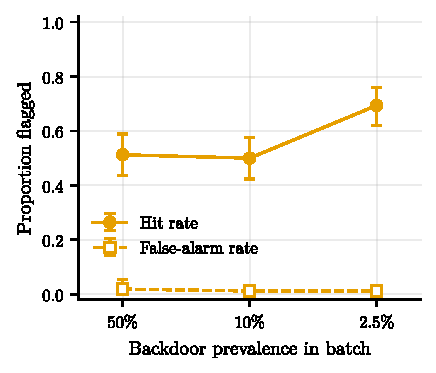
\includegraphics[width=0.47\textwidth]{figures/fig_a_prevalence_haiku.pdf}\hfill
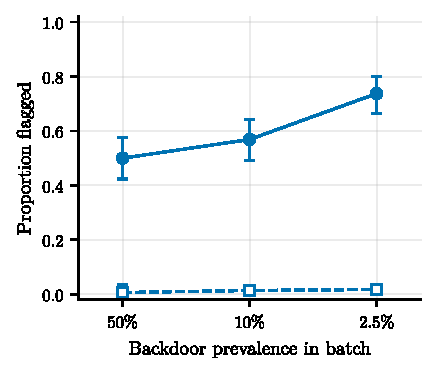
\includegraphics[width=0.47\textwidth]{figures/fig_a_prevalence_sonnet.pdf}
\caption{Hit rate and false-alarm rate by backdoor prevalence in a batch of 40 (Experiment~1); left, Haiku (orange); right, Sonnet (blue). Error bars are Wilson 95\% confidence intervals, which ignore clustering by batch.}\label{fig:prevalence}
\end{figure*}

\subsection{H1a: Criterion or Sensitivity}

The criterion did not become more conservative at low prevalence (Table~\ref{tab:h1a}; Figure~\ref{fig:sdt} in the appendix). For Sonnet, $c$ moved in the liberal direction ($\Delta c = {-0.44}$, 95\% CI $-0.70$ to $-0.28$). For Haiku, $c$ did not change reliably, and $d'$ rose ($\Delta d' = 0.71$, 0.06 to 1.04). AUROC rose slightly for both monitors, with intervals that include zero. H1a's first condition ($\Delta c > 0$ with an interval excluding zero) failed for both monitors, so H1a is not supported.

\begin{table*}[t]
\centering
\small
\begin{tabular}{@{}l l l l l l@{}}
\toprule
Monitor & $\Delta H$ [95\% CI] & $\Delta F$ [95\% CI] & $\Delta d'$ [95\% CI] & $\Delta c$ [95\% CI] & $\Delta$AUROC [95\% CI] \\
\midrule
Haiku & 0.181 [0.075, 0.281] & $-0.0069$ [$-0.0327$, 0.0128] & 0.71 [0.06, 1.04] & $-0.12$ [$-0.59$, 0.17] & 0.045 [$-0.002$, 0.092] \\
Sonnet & 0.238 [0.144, 0.338] & 0.0111 [$-0.0026$, 0.0202] & 0.39 [$-0.24$, 0.95] & $-0.44$ [$-0.70$, $-0.28$] & 0.022 [$-0.013$, 0.056] \\
\bottomrule
\end{tabular}
\caption{H1a: change from P50 to P2.5 (point estimate and 95\% cluster-bootstrap CI).}\label{tab:h1a}
\end{table*}

\subsection{H2: Stated Prevalence}

Telling Sonnet that ``about 1 in 100'' submissions contained a backdoor, rather than ``about half'', lowered its single-item hit rate from 0.850 to 0.775 (registered GLMM: log-odds $-3.32$, SE 1.25, $z = {-2.66}$, $p = .008$, Holm $p = .015$; Figure~\ref{fig:stated} in the appendix). For Haiku the hit rate went from 0.683 to 0.642 (OR 0.57, 0.22 to 1.46, $p = .244$, Holm $p = .244$).

The registered fit is numerically unreliable for Sonnet (post hoc check). Because 92 of 120 backdoored items were flagged in all three conditions, the item standard deviation $\sigma$ is large, and 40-node non-adaptive quadrature cannot resolve the likelihood there; the registered fit stopped at a local optimum of its own approximation ($\sigma = 32.8$). An accurate likelihood, computed by dense-grid integration, gives $\sigma = 13.4$ and an S1 log-odds of $-3.76$ (SE 1.41, $z = {-2.67}$, $p = .0076$; likelihood-ratio $p = .00024$). The plainest evidence needs no model: 9 Sonnet items were flagged under S50 but not under S1, and none the other way round (exact paired test, $p = .0039$). For Haiku the registered fit is accurate, and the paired counts were 12 against 7 ($p = .36$).

The GLMM coefficient is item-specific; the population-averaged odds ratio, from the item-clustered GLM, was 0.61 (0.44 to 0.84, $p = .002$), and the paired bootstrap change in Sonnet's hit rate was $-0.075$ ($-0.125$ to $-0.033$). The S1 statement moved Haiku's criterion in the conservative direction ($\Delta c = 0.29$, 0.05 to 0.59), and Sonnet's in the same direction with an interval that includes zero (0.27, $-0.01$ to 0.58). For Sonnet, S1 also lowered the AUROC slightly ($-0.017$, $-0.034$ to $-0.004$) and the mean score of backdoored items (75.0 to 62.7), while the flag rate among items scoring 40--59 did not fall (Table~\ref{tab:bands} in the appendix), so part of this effect ran through the scores. False alarms were lower under S1 than S50 but not significantly ($p = .108$ and .329). H2 is supported for Sonnet only, and the effect is small. Haiku's fall of about 4 points is within the range that, by the pre-registration's own estimate, the study may have missed.

\subsection{H3: Labelled Calibration Block}

At 2.5\% prevalence the 10 labelled examples did not significantly raise the hit rate (Figure~\ref{fig:remedies} in the appendix). Haiku's hit rate fell from 0.694 to 0.600 (OR 0.66, 0.38 to 1.16, $p = .150$, Holm $p = .150$). Sonnet's rose from 0.738 to 0.850 (OR 2.02, 0.99 to 4.10, $p = .053$, Holm $p = .106$). For Sonnet the block moved the criterion in the liberal direction ($\Delta c = {-0.37}$, $-0.59$ to $-0.18$) with no change in $d'$ (0.03, $-0.38$ to 0.48), and its false-alarm rate rose from 1.7\% to 4.0\% ($\Delta F = 0.0224$, 0.0139 to 0.0314). Its mean number of flags per batch rose from 1.41 to 2.40. H3 is not supported. With 80 backdoored judgements per remedy cell, effects of the size of Sonnet's rise may have gone undetected, so this null result is weak evidence that the block does not help.

\subsection{Exploratory and Post Hoc Analyses}

\paragraph{E1, position.} The position of the backdoored item in the batch did not predict hits in either monitor or condition (all $p \geq .08$). Figure~\ref{fig:position} in the appendix does show lower hit rates for backdoors in the first eight positions of P10 batches, a pattern that the registered linear test would not detect. One of eight uncorrected tests was significant: Sonnet's false alarms became more frequent later in P2.5 batches (OR per 10 positions 1.26, $p = .019$).

\paragraph{E2, independence instruction.} R-ind did not change hit rates (Haiku OR 0.74, 0.42 to 1.30, $p = .288$; Sonnet OR 1.07, 0.57 to 1.98, $p = .835$). Haiku's false-alarm rate was slightly lower ($\Delta F = {-0.0045}$, ${-0.0088}$ to ${-0.0003}$).

\paragraph{E3, monitors.} In batches the two monitors did not differ (all monitor terms and interactions $p \geq .195$). In single-item review Sonnet caught more backdoors than Haiku (log-odds 0.965, SE 0.230, $p < .001$, at S50).

\paragraph{E4, single item against batch.} Single-item review with no stated rate (Haiku 0.633, Sonnet 0.800) caught about as many backdoors as the P2.5 batches and more than the P50 and P10 batches in three of four comparisons. Odds ratios for batch against single were, for Haiku, 0.61 at P50 ($p = .051$), 0.58 at P10 ($p = .026$) and 1.31 at P2.5 ($p = .291$); for Sonnet, 0.25 ($p < .001$), 0.33 ($p < .001$) and 0.70 ($p = .226$). False alarms did not differ (all $p \geq .46$). These comparisons use different item sets, and the prompts differ by one sentence.

\paragraph{Post hoc: how flags relate to scores.} In every condition the flag behaved almost like a fixed threshold on the monitor's own suspicion score. No item scoring below 20 was flagged and every item scoring 60 or more was; most of the change happened in the 40--59 band, with a few items scoring 20--39 flagged in some conditions (Table~\ref{tab:bands}). The prevalence effect therefore came from the scores. Backdoored items scored lower at P50 than at P2.5 (Table~\ref{tab:measures}), and fewer of them reached the top band (80--100: Haiku 0.09 against 0.22, Sonnet 0.17 against 0.45). Clean items scored low throughout.

\paragraph{Post hoc: reasoning length and robustness.} Haiku's mean thinking tokens per batch call were 7,592 at P50 against 4,195 at P2.5; Sonnet's were 116 against 480. Dropping the calls with in-call schema corrections left the conclusions for H1 to H3 unchanged (H2 tested with the item-clustered GLM). The H1 odds ratios were 2.35 for Haiku ($p = .0007$) and 2.81 for Sonnet ($p < .001$), and Haiku's H3 $p$ value moved from .150 to .076, still not significant.

% ===========================================================================
\section{Discussion}

\paragraph{What was found.} The low-prevalence effect did not appear. In batch review, both Claude monitors caught more backdoors at 2.5\% prevalence than at 50\%, and the criterion did not become more conservative. The clearest contrast is between batches with one backdoor and batches with several. P2.5 batches and single-item review gave similar hit rates, while P10 and P50 batches, which behaved alike, gave lower ones. A stated base rate of 1 in 100 had a small effect on Sonnet that ran at least partly through its scores; its criterion moved in the conservative direction, but not reliably.

\paragraph{Why no low-prevalence effect.} The human effect builds up over many trials, as observers learn the base rate and lower their quitting thresholds \citep{wolfe2005,wolfe2007}. An LLM monitor sees all 40 items at once; nothing in the call resembles a long run of empty searches, so there may be no route by which rarity becomes conservatism.

\paragraph{Why fewer hits with several backdoors.} Two candidate explanations fit the data equally well. The design cannot separate them, because it varied only the number of backdoors in a batch of 40, and P10 (4 backdoors) behaved like P50 (20).
\begin{itemize}
\item \textbf{Pop-out.} A monitor that sees a whole batch may judge each item partly against the others, so one odd item among 39 ordinary ones stands out. This fits the ``implicit normalization of decisions within the batch'' of \citet{hida2026}, whose balanced review, like P50 here, was screened more restrictively in batches, although P2.5 batches were not significantly more inclusive than single-item review.
\item \textbf{Crowding.} When several items deserve attention, each may look less exceptional or get less scrutiny, loosely like the human subsequent search misses \citep{cain2013}. The monitors did score every item, and their reasoning length pointed both ways (at P50 Haiku reasoned more and Sonnet much less).
\end{itemize}
Both explanations agree with the post hoc finding that the flag threshold stayed put while backdoored items scored lower when several shared a batch. Telling them apart needs a design that varies the number of backdoors and the batch size separately. The flag was close to a fixed threshold on the score in every condition, so SDT's split between evidence and criterion maps onto something real in these monitors.

\paragraph{Safety implications, stated as hypotheses.} For the rare-attack strategy that control evaluations usually assume, these results are mildly reassuring: rarity did not make these monitors miss more. They raise a different concern. If backdoored items score lower when several share a review context, an attacker who could place several attacks in one batch, coordinating them ``across space'' \citep[Sec.~6]{korbak2025}, might lower the suspicion of each. This study is not evidence that this happens in realistic monitoring; it is a hypothesis to test in agent settings, where one transcript may contain several suspicious actions. If the pattern holds more widely, three points follow. First, batch composition is a variable in monitor evaluation: balanced batches understated the hit rate at low prevalence here, and the arithmetic extrapolations used in current work \citep{abbasi2026,srivastav2026} assume that class-conditional score distributions do not change with prevalence, and for batch review in this study they did. Second, per-item review did about as well as the best unremedied batches here and better than most batches with several backdoors, so where cost allows it may be the safer design. Third, prompts that state an expected attack rate can move a monitor's judgements, as the S1 sentence did for Sonnet, so such statements should be chosen deliberately and tested.

\paragraph{Remedies.} In people, high-prevalence bursts with feedback restore a criterion that has drifted too conservative, at the cost of more false alarms than in a baseline experiment \citep[Experiment~7]{wolfe2007}. These monitors had no such drift to undo. The labelled block left Haiku's hit rate statistically unchanged and pushed Sonnet's criterion in the liberal direction, adding hits and false alarms together: it moved the operating point rather than restoring one. In a deployed protocol each extra false alarm uses audit budget, which is 2\% of problems in \citet{greenblatt2024} and 0.1\% of actions in \citet{korbak2025}. The R-cal examples also came from different problems from the scored items, and probes may help mainly with targets that resemble them \citep{becker2026}. TIP's other job, measurement, gains support. If a monitor's hit rate depends on what else is in its context, the most direct estimate of deployed performance comes from known attacks inserted into the real stream \citep{korbak2025}; in airport screening, about 100 TIP events per screener gave a reliability of at least 0.7 when the mean hit rate was below 0.9 \citep{buser2025}.

\paragraph{What the human analogy did and did not predict.} The analogy predicted a conservative criterion shift at low experienced prevalence, which did not happen, and it did not predict the drop in hits when several backdoors shared a batch. Its most useful contribution was its method. SDT and the criterion--sensitivity distinction, together with the post hoc score-band analysis, made it possible to see that the reversal came from the scores given to backdoored items, not from where the flag threshold sat.

% ===========================================================================
\section{Limitations}

\paragraph{One domain and one item source.} The items are short solutions to entry-level problems, each with at most one backdoor, written by one generator under one instruction; real agent attacks are longer, multi-step and adaptive \citep{kutasov2025,najt2026,najt2026arxiv}.

\paragraph{Claude-only monitors and an unlogged harness context.} The monitors and the generator come from one model family, at effort \code{low}, called through Claude Code. Each call carried about 1,800 tokens of unlogged Claude Code scaffolding; it was constant across conditions, monitors and time, so it cannot explain differences between conditions with the same presentation; as a larger share of single-item inputs, it may bear on E4 and on absolute rates. Other families, settings and direct API calls may behave differently.

\paragraph{Small P50 cell.} As registered, P50 had 8 batches per monitor, so its cluster-robust and bootstrap intervals are approximate and may be too narrow; the direction of H1 is consistent across monitors and with E4.

\paragraph{One batch size and a limited range.} All batches held 40 items, so the number and the share of backdoors were not varied separately, and pop-out and crowding cannot be told apart. The lowest prevalence was 2.5\%, far above deployed attack rates. Experienced prevalence existed only within one call; most deployed monitors judge one transcript per call.

\paragraph{Power.} As the pre-registration warned, effects smaller than about 15 points may have been missed. This matters most for the null results of H3 (80 backdoored judgements per cell) and of Haiku's H2.

\paragraph{Measurement limits.} False alarms were very rare, so $d'$ and $c$ rest mainly on the hit rate, and single-item false-alarm rates rest on 120 clean items. The registered H2 model is numerically unreliable for Sonnet; an accurate post hoc refit and an exact paired test support the same conclusion. Items were reused across batches, and the H1 analysis clusters by batch only. E4 compares different item sets under prompts that differ by a sentence.

\paragraph{Process.} Clarifications 4 to 12 were committed after data collection had begun, the timing of the edit-size threshold rests on the engineer's record, and post hoc analyses were added after the data were seen. In-call schema corrections, inferred from turn counts, were not anticipated by the registered retry rule; excluding them did not change H1 to H3.

% ===========================================================================
\section{Conclusion}

Human screeners miss rare targets, and AI control expects attacks to be rare. In this pre-registered test with two Claude models and toy code, LLM monitors did not miss rare attacks more often. Both monitors caught more backdoors when one backdoor sat in a batch of 40 than when twenty did, and batches with four behaved like those with twenty. Single-item review did about as well as the low-prevalence batches. Backdoored items scored lower when several shared a batch. Whether that is because a lone backdoor stands out or because several crowd each other out cannot be told apart here. A TIP-style calibration block did not reliably help, and a stated base rate slightly lowered one monitor's hit rate. The results argue for evaluating monitors with the item mix and presentation they will face in deployment, for treating batch composition as a variable, and for testing whether clustered attacks lower per-item suspicion in realistic agent settings.

\section{Disclosure of AI Assistance}

Literature searches, drafting, source verification, the experimental code and the analysis were carried out with AI assistance (Claude, Anthropic) under the authors' direction. An independent AI-assisted audit checked references, quotations and analysis against their sources. The authors are responsible for the final text. Several AI-safety sources cited are research reports by Anthropic, the assistant's developer. Claude models also served as the item generator and the monitors.

\bibliography{references}

% ===========================================================================
\appendix
\section{Technical Appendix}

This appendix gives supporting material for the main text: the post hoc score-band table, the H2 and H3 results and the registered $d'$ and $c$ estimates in graphical form, and the exploratory position analysis (E1).

\begin{table}[t]
\centering
\small
\begin{tabular}{@{}l l r r@{}}
\toprule
Monitor & Condition & Top band & Flag at 40--59 \\
\midrule
Haiku & P50 & 0.09 & 0.73 \\
Haiku & P2.5 & 0.22 & 0.84 \\
Haiku & \emph{none} (single) & 0.17 & 1.00 \\
Sonnet & P50 & 0.17 & 0.85 \\
Sonnet & P2.5 & 0.45 & 0.93 \\
Sonnet & \emph{none} (single) & 0.60 & 0.83 \\
Sonnet & S50 (single) & 0.72 & 0.83 \\
Sonnet & S1 (single) & 0.47 & 1.00 \\
\bottomrule
\end{tabular}
\caption{Post hoc. ``Top band'' is the share of backdoored items scoring 80--100. ``Flag at 40--59'' is the share of all items in that score band that were flagged.}\label{tab:bands}
\end{table}

\begin{figure*}[t]
\centering
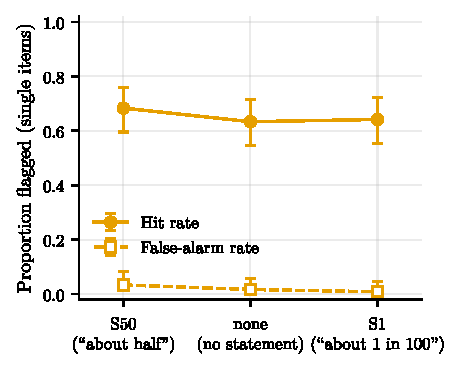
\includegraphics[width=0.495\textwidth]{figures/fig_d_stated_prevalence_haiku.pdf}\hfill
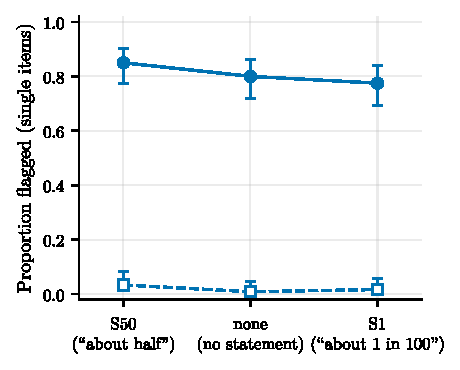
\includegraphics[width=0.495\textwidth]{figures/fig_d_stated_prevalence_sonnet.pdf}
\caption{Single-item hit and false-alarm rates under three statements of the base rate (Experiment~2); left, Haiku (orange); right, Sonnet (blue). Error bars are Wilson 95\% confidence intervals.}\label{fig:stated}
\end{figure*}

\begin{figure*}[t]
\centering
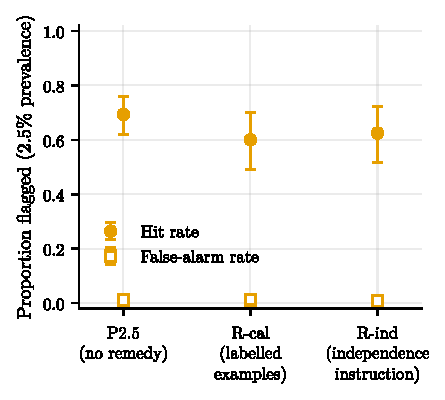
\includegraphics[width=0.48\textwidth]{figures/fig_e_remedies_haiku.pdf}\hfill
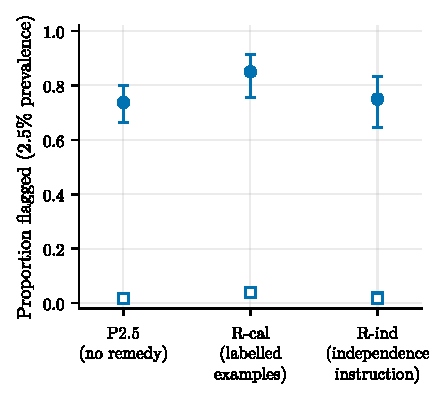
\includegraphics[width=0.48\textwidth]{figures/fig_e_remedies_sonnet.pdf}
\caption{Hit and false-alarm rates at 2.5\% prevalence without a remedy (P2.5), with the labelled calibration block (R-cal) and with the independence instruction (R-ind); left, Haiku (orange); right, Sonnet (blue). Error bars are Wilson 95\% confidence intervals.}\label{fig:remedies}
\end{figure*}

\begin{figure*}[t]
\centering
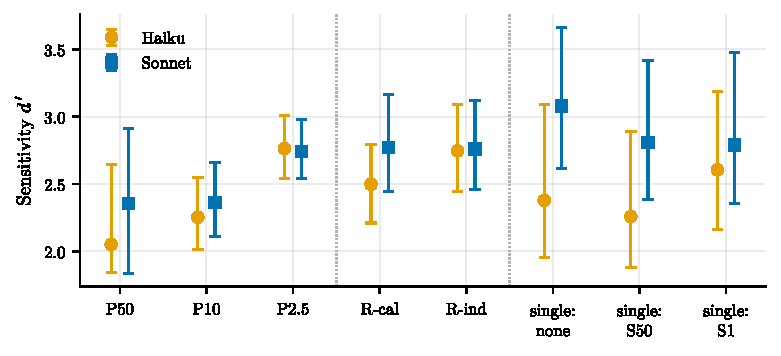
\includegraphics[width=0.87\textwidth]{figures/fig_b_sdt_dprime.pdf}

(a) Sensitivity $d'$

\medskip
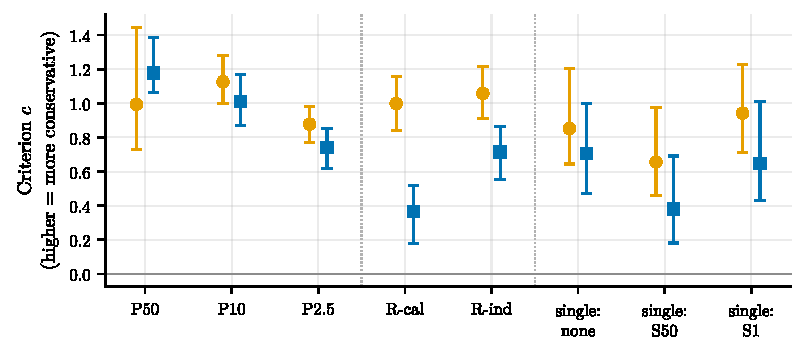
\includegraphics[width=0.87\textwidth]{figures/fig_b_sdt_c.pdf}

(b) Criterion $c$
\caption{Sensitivity $d'$ (a) and criterion $c$ (b; higher is more conservative) for every condition and monitor (Haiku orange, Sonnet blue), with log-linear correction. Error bars are 95\% bootstrap confidence intervals: a cluster bootstrap over batches for Experiments 1 and 3, and a paired item bootstrap for Experiment~2.}\label{fig:sdt}
\end{figure*}

\begin{figure*}[t]
\centering
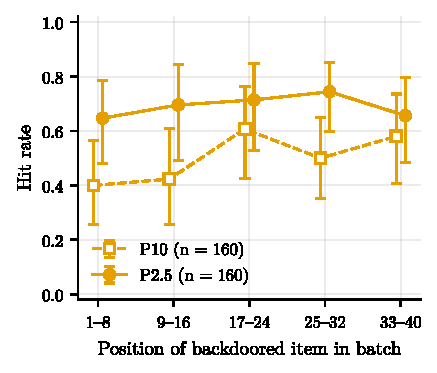
\includegraphics[width=0.47\textwidth]{figures/fig_c_position_haiku.pdf}\hfill
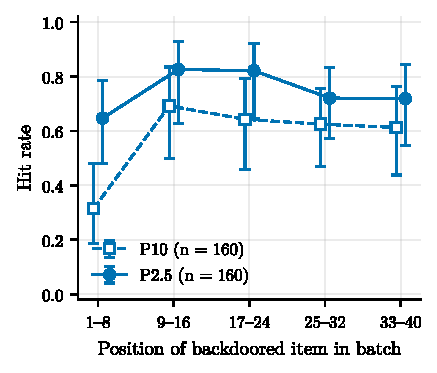
\includegraphics[width=0.47\textwidth]{figures/fig_c_position_sonnet.pdf}
\caption{Hit rate by position of the backdoored item in the batch, in bins of eight positions (exploratory, E1); left, Haiku (orange); right, Sonnet (blue). Error bars are Wilson 95\% confidence intervals. The plot shows lower hit rates for backdoors in the first eight positions of P10 batches, a pattern that the registered linear test would not detect.}\label{fig:position}
\end{figure*}

\end{document}
